\begin{table}[]
\resizebox{\columnwidth}{!}{
\centering
\begin{tabular}{c|c|c|c|c|c|c|}
\cline{2-7}
                                                                                     & \multicolumn{6}{c|}{\textbf{Number of Actions in Execution Path}}                                 \\ \hline
\multicolumn{1}{|c|}{\textbf{Planner}}                                               & \textbf{S1} & \textbf{S2} & \textbf{S3} & \textbf{S4} & \textbf{S5} & \textbf{S6} \\ \hline
\multicolumn{1}{|c|}{PokeRRT*}                                                       & 
\textbf{\begin{tabular}[c]{@{}c@{}}3.93\\ (0.98)\end{tabular}} & \textbf{\begin{tabular}[c]{@{}c@{}}4.62\\ (1.04)\end{tabular}}                       
&   \textbf{\begin{tabular}[c]{@{}c@{}}4.49\\ (1.02)\end{tabular}}   
&   \textbf{\begin{tabular}[c]{@{}c@{}}4.76\\ (1.20)\end{tabular}}   
& \textbf{\begin{tabular}[c]{@{}c@{}}3.71\\ (1.02)\end{tabular}} &  \textbf{\begin{tabular}[c]{@{}c@{}}3.65\\ (1.08)\end{tabular}}\\ \hline
\multicolumn{1}{|c|}{PokeRRT} &
  \begin{tabular}[c]{@{}c@{}}6.10 \\ (1.96)\end{tabular} &
\begin{tabular}[c]{@{}c@{}}8.21\\ (2.95)\end{tabular}  &
\begin{tabular}[c]{@{}c@{}}7.94\\ (2.08)\end{tabular}  &\begin{tabular}[c]{@{}c@{}}6.77\\ (2.35)\end{tabular}
  &
\begin{tabular}[c]{@{}c@{}}4.56\\ (1.27)\end{tabular}  &
 \begin{tabular}[c]{@{}c@{}}8.17\\ (2.46)\end{tabular} \\ \hline
\multicolumn{1}{|c|}{\begin{tabular}[c]{@{}c@{}}LI-PokeRRT*\end{tabular}} & 
\begin{tabular}[c]{@{}c@{}}16.43\\ (2.28)\end{tabular}&
\begin{tabular}[c]{@{}c@{}}22.27\\ (2.26)\end{tabular}
&\begin{tabular}[c]{@{}c@{}}19.00\\ (1.54)\end{tabular}
&\begin{tabular}[c]{@{}c@{}}18.54\\ (1.44)\end{tabular}
&N/A
& N/A            \\ \hline

\multicolumn{1}{|c|}{\begin{tabular}[c]{@{}c@{}}LI-PokeRRT\end{tabular}} &
\begin{tabular}[c]{@{}c@{}}19.08 \\ (1.51)\end{tabular}
  &
\begin{tabular}[c]{@{}c@{}}19.62\\ (1.64)\end{tabular}  &
 \begin{tabular}[c]{@{}c@{}}20.74\\ (2.13)\end{tabular} &\begin{tabular}[c]{@{}c@{}}19.38\\ (1.59)\end{tabular}
  &
N/A  &
N/A  \\ \hline
\multicolumn{1}{|c|}{\begin{tabular}[c]{@{}c@{}}Push Planner\end{tabular}} &
\begin{tabular}[c]{@{}c@{}}8.72 \\ (1.42)\end{tabular} &
\begin{tabular}[c]{@{}c@{}}8.61\\ (1.71)\end{tabular}   &
\begin{tabular}[c]{@{}c@{}}7.68\\ (1.19)\end{tabular}   &\begin{tabular}[c]{@{}c@{}}8.53 \\ (1.51)\end{tabular}
  &N/A
   &N/A
   \\ \hline\hline
\multicolumn{1}{|c|}{Pick-and-Place}                                                 & \begin{tabular}[c]{@{}c@{}}1.00\\ (0.00)\end{tabular}           & \begin{tabular}[c]{@{}c@{}}1.00\\ (0.00)\end{tabular}           & \begin{tabular}[c]{@{}c@{}}1.00\\ (0.00)\end{tabular}           & N/A           & \begin{tabular}[c]{@{}c@{}}1.00\\ (0.00)\end{tabular}           & N/A           \\ \hline
\end{tabular}
}
\caption{Number of executed actions in the planned path for various algorithms in simulation are presented here. Both \textsl{PokeRRT*} and  \textsl{Low-Impulse PokeRRT*} lead to fewer actions than their RRT-based counterparts, thus exploiting the large displacement property inherent to poking manipulation.\vspace{-12pt}}
\label{tab:eval-sim-actions}
\end{table}

\subsection{Simulation Experiments}

\cref{tab:eval-sim-time} shows the task times and success rates for \textsl{Pick-and-Place} and five non-prehensile manipulation planners---\textsl{PokeRRT*},  \textsl{Low-Impulse PokeRRT*},  \textsl{PokeRRT},  \textsl{Low-Impulse PokeRRT}, and \textsl{Two-Level Push Planner}. Results are averaged over 250 trials. \textsl{PokeRRT} and \textsl{PokeRRT*} successful in all scenarios while \textsl{Two-Level Push Planner} fails in S5 and S6 and grasping fails in S4 and S6. \textsl{Two-Level Push Planner} has a low overall success rate ($44\%$), as expected based on the reasons presented in \cref{sec:evaluation-scenarios}.

\textsl{PokeRRT} and \textsl{PokeRRT*} task times are lower than \textsl{Two-Level Push Planner} task times across all scenarios. Standard deviations are high due to the sampling-based nature of our planners. The task time for S4 is greater than for S1 since the object used in S4 is not only bigger in size but also larger in mass than the object used in S1, therefore poke displacements are lower given the same contact force. \textsl{Pick-and-Place} has the lowest task time because it does not involve planning in the object configuration space---the robot moves to object pose, grasps, and moves to goal pose, so only a single action is executed. Low-impulse poke planners have large search trees due to shorter displacements of the object. This results in longer planning times and also lower success rates. Task times are higher for obstacle scenarios because the robot end-effector is more likely to run into obstacles and collision checking is a computationally expensive procedure.

\textsl{Pick-and-Place} succeeds in simulation for S1, S2, S3, and S5 because there is no uncertainty in object pose so manipulation consists of moving to a predefined grasp configuration and moving to the goal pose. We intentionally set up the start and goal configurations for \textsl{Pick-and-Place} to create an upper bound for comparison with our planners. For the reasons presented in \cref{sec:evaluation-scenarios}, it fails in S4 and S6. Low-impulse poke planners have higher success rates than the push planner because the shorter robot control trajectories corresponding to poking result in fewer obstacle collisions. Low-impulse poke planners fail in S5 and S6 because the pokes are not strong enough to pass the workspace divider or cross into the second robot's reachable workspace.

% \begin{figure}
%   \centering
%     \includegraphics[width=\linewidth]{figures/sampleplans}
%   \caption{Plans generated by \textsl{PokeRRT} (a) involve more pokes than those generated by \textsl{PokeRRT*} (b), which indicates that \textsl{PokeRRT*} is better able to exploit poking's key characteristic of covering large distances.\vspace{-28pt}}\label{fig:plans}
% \end{figure}
% \vspace{-4.5pt}
\cref{tab:eval-sim-actions} presents the number of executed actions in the final planned path for multiple planning algorithms across several scenarios. It indicates that the number of executed actions is lower for \textsl{PokeRRT} and \textsl{PokeRRT*} compared to \textsl{Two-Level Push Planner}, showing that poke planners can displace the object further with fewer actions in less time. Notably, the number of actions is lowest for \textsl{PokeRRT*}, thereby supporting our claim that minimizing the number of poking actions exploits the large displacement property of poking manipulation.
% (\cref{fig:plans}).
However, the task time is similar to that of \textsl{PokeRRT} since \textsl{PokeRRT*} introduces the choose parent and rewiring steps to \textsl{PokeRRT}, which increases the number of actions sampled while planning. In general, \textsl{PokeRRT} is preferable in scenarios with obstacles---even though the number of pokes for \textsl{PokeRRT*} is lower (i.e., faster overall execution), a greater percentage of time is spent on resampling actions in \textsl{PokeRRT*}, most of which lead to object--obstacle collisions. Task times for low-impulse poke planners are comparable to \textsl{Two-Level Push Planner}, supporting our claim that pushing is a limiting case of poking where applied impulses are low in magnitude.

\begin{figure}
\vspace{4pt}
  \centering
    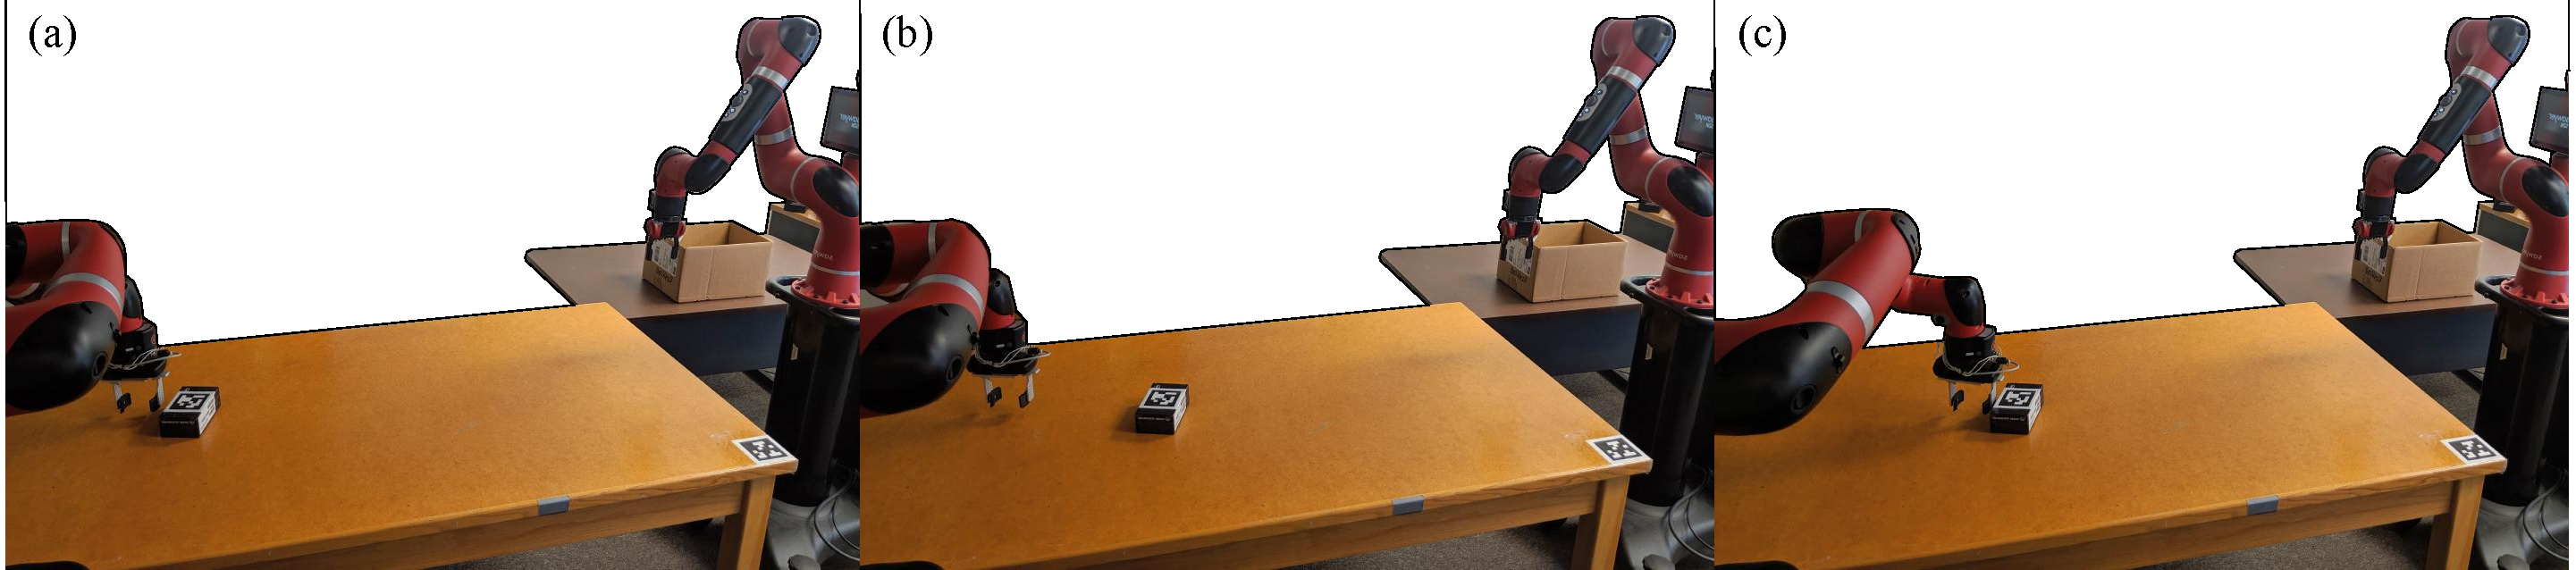
\includegraphics[width=\linewidth]{figures/vignette1-min.pdf}\\
    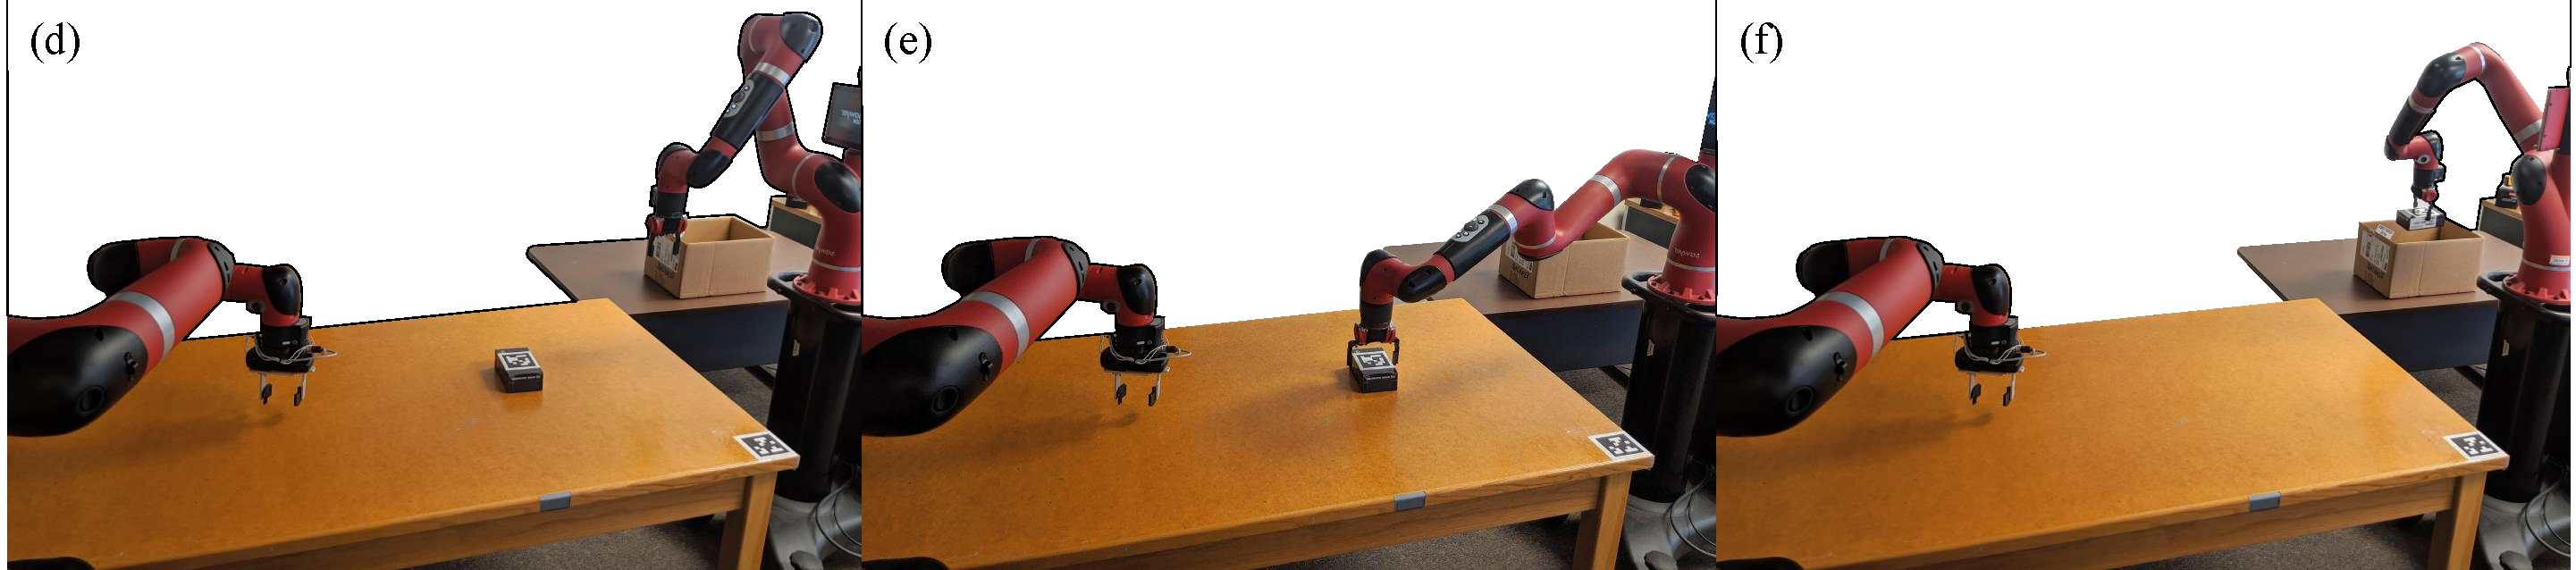
\includegraphics[width=\linewidth]{figures/vignette2-min.pdf}
  \vspace{-12pt}
  \caption{Two robots with non-overlapping reachable regions are shown (S6). Robot A (left) applies 2 pokes to manipulate the object to Robot B's (right) workspace (a-d). Robot B then grasps the object and places it in a bin that is not reachable by Robot A (e-f).\vspace{-15pt}}\label{fig:vignette}
\end{figure}

\subsection{Real-World Experiments}

We evaluate \textsl{PokeRRT*}, \textsl{PokeRRT}, \textsl{Two-Level Push Planner}, and \textsl{Pick-and-Place} for a subset of the scenarios in the real-world (\cref{tab:eval-real}). The task times and the number of actions executed in the real world are slightly higher than in simulation. This is expected because the plan is generated in simulation and simulation does not fully capture the complexities of the real-world environment. Therefore, replanning is required for real-world plan execution which leads to an increase in task times. As shown in \cref{fig:plot}, execution times for poke planners are lower than for the push planner indicating that poke planning leads to faster object manipulation than push planning. Additionally, the replanning time for push planning is higher than for poke planning since simulating push actions to generate the planning graph takes more computational cycles than simulating instantaneous contact for poke actions. However, the number of replans for push planning is lower than for poke planning thereby pointing to the inherently uncontrollable nature of poking, which may not be desirable in certain situations (\cref{tab:eval-real}).
Collectively, real-world results align with the results from simulation.
% Similar to simulation results, \textsl{PokeRRT*} has the fewest number of executed actions. In S4, poking is 1.7 times faster than pushing. In S5, pushing fails because of collision with obstacles and grasping fails because the object is too large for the gripper. Both pushing and grasping fail in S6 because the goal region is unreachable.

\cref{fig:vignette} depicts a failure recovery case for S6 where failure to grasp or push to the second robot's reachable workspace does not result in task failure---the first robot pokes the object to the second robot's reachable workspace, allowing the second robot to successfully manipulate the object.
Additionally, while grasping is a faster form of manipulation with fewer actions than poking or pushing, it has a lower overall success rate ($27\%$) than pushing ($33\%$) due to perception inaccuracies. This discrepancy between simulation and real-world results points to a fundamental difference between grasping and poking or pushing---sensing uncertainty leads to total failure in grasping, whereas for poking it leads to just partial failure as our presented planners operate in a closed-loop manner. 
